\documentclass{article}
\usepackage{amsmath}
\usepackage{amssymb}
\usepackage{tikz}
\usepackage{array}
\usepackage{pgfplots}
\pgfplotsset{compat=1.18}
\usepackage[utf8]{inputenc}
\usepackage{ragged2e} % Pour la justification
\usepackage{geometry}
\usepackage{float}



% Ajuster les marges de la page
\geometry{
    a4paper,
    left=2cm,
    right=2cm,
    top=2cm,
    bottom=2cm
}


\begin{document}



% Titre stylé
\begin{center}
    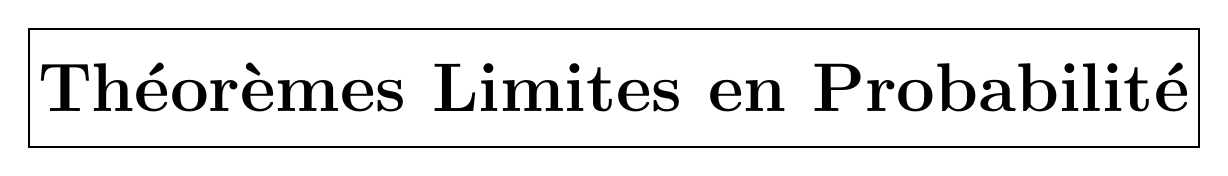
\begin{tikzpicture}
        \node[draw, thick, minimum width=12cm, minimum height=1.5cm, align=center] at (0,0) {\Huge \textbf{\textsc{Théorèmes Limites en Probabilité}}};
    \end{tikzpicture}
\end{center}

\vspace{0.1cm}

\begin{justify}
Historiquement, la théorie des probabilités a d'abord commencé à s'élaborer autour des phénomènes aléatoires les plus simples, c'est-à-dire : les jeux de hasard. 
Ainsi, grâce aux possibilités de répétition des mêmes expériences qu'ils offrent, les jeux de hasard ont d'abord permis, de manière très simple, d'étudier certains phénomènes ; puis d'émettre certaines hypothèses.
\end{justify}


\begin{justify}
\noindent En effet, il suffit de lancer une pièce un très grand nombre de fois pour s'apercevoir que chacune des faces de la pièce a une fréquence d'apparition d'environ $1/2$. Et c'est dans ce contexte précis, que trois siècles plus tôt, J. Bernoulli énonce pour la première fois la loi des grands nombres.
\end{justify}



\begin{justify}
\noindent Une fois le formalisme établi, nos lancers de pièces équilibrées laissent place à un m-échantillon $(X_1, \dots, X_m)$ de variables aléatoires i.i.d de distribution de Bernoulli $\mathcal{B}(1/2)$ et $\forall i \in \{1, \dots, m\}$, $X_i = 1$ si pile et $0$ si face avec ici chaque $X_i$ qui représente le résultat du i-ème lancer de pièce.
\end{justify}



\begin{justify}
\noindent
Considérons une suite $(X_n)_{n \in \mathbb{N}}$ de variables aléatoires i.i.d, de carré intégrable, c'est-à-dire $\mathbb{E}(X_1^2) < +\infty$ et $\mathbb{E}(X_1) = m$.

\noindent Alors la moyenne empirique : $\overline{X}_m = \frac{1}{m} \sum_{i=1}^{m} X_i$ converge vers $m$.

\noindent Sous ces hypothèses, la manière dont on définira le mode de convergence opérera la distinction entre loi forte et loi faible des grands nombres.
\end{justify}

\begin{justify}
\noindent
D'autres théorèmes affinent l'énoncé de cette loi (LGN) comme le théorème central limite (TCL) et la loi du logarithme itéré qui précisent la vitesse de convergence de $\overline{X}_m$, ou bien encore la loi du 0-1 de Kolmogorov qui étudie le comportement asymptotique des séquences de variables aléatoires. Le but de cet exposé sera donc d’étudier la LGN ainsi que certains de ses raffinements en détail.
\end{justify}

\begin{justify}
\noindent
La loi des grands nombres s'énonce de la manière suivante :
\end{justify}

\vspace{0.1cm}

\section*{\underline{Loi faible des grands nombres}}


\textbf{Théorème :} Soit $(X_n)_{n \in \mathbb{N}^*}$ une suite de variables aléatoires réelles intégrables, indépendantes et de même loi. Soit $m$ leur espérance commune.

\vspace{0.3cm}
On note pour $m \in \mathbb{N}^*$ :

\[
S_m = X_1 + \cdots + X_m \quad \text{et} \quad \frac{S_m}{m} = \frac{X_1 + \cdots + X_m}{m}
\]

Alors la suite $\left(\frac{S_m}{m}\right)_{m \in \mathbb{N}^*}$ tend vers $m$ en probabilité :

\[
\forall \varepsilon > 0, \quad \lim_{m \to \infty} \mathbb{P}\left(\left|\frac{S_m}{m} - m\right| \geq \varepsilon\right) = 0
\]

D'où :

\[
\mathbb{P}(|X| \geq \varepsilon) \leq \frac{\mathbb{E}(|X|)}{\varepsilon}
\]

\begin{justify}
Pour démontrer la loi faible des grands nombres, nous nous limitons à considérer des variables aléatoires dont le moment d'ordre 1 est intégrable. Pour cela, nous employons l'inégalité de Bienaymé-Tchebychev, elle-même conséquence de l'inégalité de Markov.
\end{justify}

\section*{\underline{Inégalité de Markov}}


\textbf{Théorème :} Soit $X$ une variable aléatoire réelle et intégrable, alors, pour tout $\varepsilon > 0$ :

\[
\mathbb{P}(|X| \geq \varepsilon) \leq \frac{\mathbb{E}(|X|)}{\varepsilon}
\]

\vspace{1cm}
\noindent
\textbf{Démonstration :}

\vspace{0.3cm}
\noindent
Soit $\varepsilon > 0$, alors :

\[
\mathbb{E}(|X|) = \mathbb{E}(|X| \cdot \mathbf{1}_{|X| \geq \varepsilon}) + \mathbb{E}(|X| \cdot \mathbf{1}_{|X| < \varepsilon})
\]

\[
\geq \mathbb{E}(\varepsilon \cdot \mathbf{1}_{|X| \geq \varepsilon}) + 0
\]

\[
\geq \varepsilon \cdot \mathbb{E}(\mathbf{1}_{|X| \geq \varepsilon}) + 0
\]

\[
= \varepsilon \cdot \mathbb{P}(|X| \geq \varepsilon)
\]

\section*{\underline{Inégalité de Bienaymé-Tchebychev}}



\textbf{Théorème :} Soit $X$ une variable aléatoire de carré intégrable, alors :

\[
\forall \varepsilon > 0, \quad \mathbb{P}(|X - \mathbb{E}(X)| \geq \varepsilon) \leq \frac{\text{Var}(X)}{\varepsilon^2}
\]

\vspace{1cm}
\noindent
\textbf{Démonstration :}

\vspace{0.3cm}
\noindent
On observe que l'événement $\{|X - \mathbb{E}(X)| \geq \varepsilon\}$ est égal à l'événement $\{(X - \mathbb{E}(X))^2 \geq \varepsilon^2\}$. En appliquant l'inégalité de Markov à la variable aléatoire $(X - \mathbb{E}(X))^2$ et au nombre $\varepsilon^2$, on obtient :

\[
\mathbb{P}(|X - \mathbb{E}(X)| \geq \varepsilon) = \mathbb{P}((X - \mathbb{E}(X))^2 \geq \varepsilon^2)
\]

\[
\leq \frac{\mathbb{E}((X - \mathbb{E}(X))^2)}{\varepsilon^2}
\]

\[
= \frac{\text{Var}(X)}{\varepsilon^2}
\]

\vspace{1cm}
\noindent
\textbf{Démonstration de la loi faible des grands nombres :}

\vspace{0.3cm}
\noindent
Soit $\varepsilon > 0$, alors en appliquant l'inégalité de Bienaymé-Tchebychev à la variable aléatoire $\left| \frac{S_m}{m} - m \right|$ et au nombre $\varepsilon$, on obtient :

\[
\mathbb{P}\left(\left| \frac{S_m}{m} - m \right| \geq \varepsilon\right) = \mathbb{P}\left(\left| \frac{X_1 + \cdots + X_m}{m} - m \right| \geq \varepsilon\right) \leq \frac{\text{Var}\left(\frac{X_1 + \cdots + X_m}{m}\right)}{\varepsilon^2}
\]

Or,

\[
\text{Var}\left(\frac{X_1 + \cdots + X_m}{m}\right) = \frac{1}{m^2} \cdot \text{Var}(X_1 + \cdots + X_m)
\]

\[
\leq \frac{\text{Var}(X_1 + \cdots + X_m)}{m^2 \varepsilon^2}
\]

Comme $X_1, \ldots, X_m$ sont des variables aléatoires indépendantes et de même loi, on a :

\[
\text{Var}(X_1 + \cdots + X_m) = \text{Var}(X_1) + \cdots + \text{Var}(X_m) = m \cdot \text{Var}(X_1)
\]

Donc,

\[
0 \leq \mathbb{P}\left(\left| \frac{S_m}{m} - m \right| \geq \varepsilon\right) \leq \frac{\text{Var}(X_1)}{m \cdot \varepsilon^2}
\]

D'où :

\[
\lim_{m \to \infty} \mathbb{P}\left(\left| \frac{S_m}{m} - m \right| \geq \varepsilon\right) = 0
\]

\vspace{1cm}

\begin{justify}
\noindent
On souhaiterait désormais démontrer la loi forte. Cependant, nous n'avons pas encore tous les outils pour le faire. C'est pourquoi nous allons d'abord renforcer notre arsenal et cela passe entre autres en premier lieu par l'étude d'un nouveau raffinement des théorèmes limites classiques.
\end{justify}

\begin{justify}
\noindent
Pour cela, reprenons l'exemple présenté en introduction (celui du lancer de pièces équilibrées).

\noindent
Pour rappel, on avait un échantillon $(X_1, \ldots, X_n)$ de variables identiques, indépendantes et de distribution de Bernoulli. On sait désormais que :

\[
\overline{X}_n = \frac{1}{n} \sum_{i=1}^n X_i \quad \text{converge vers } \frac{1}{2} \text{ en probabilité grâce à la loi faible des grands nombres.}
\]

\noindent
Notons $E$ l'événement : "la fréquence des piles dans la série de lancers converge vers $0,5$ lorsque le nombre de lancers tend vers l'infini".

\vspace{0.5cm}
\noindent
La loi du 0-1 de Kolmogorov nous indique que $E$ se réalisera presque sûrement avec probabilité 1 ou presque jamais avec probabilité 0. Globalement, cette loi donne des informations plus précises sur le comportement asymptotique des séquences aléatoires. Formellement, elle se présente comme suit: 
\end{justify}

\section*{\underline{Loi du 0-1 de Kolmogorov}}

Soit $(\Omega, \mathcal{A}, \mathbb{P})$ un espace probabilisé.  
Soit $(X_n)_{n \in \mathbb{N}}$ des variables aléatoires sur $(\Omega, \mathcal{A}) \rightarrow (\mathbb{R}, \mathcal{B}_\mathbb{R})$, indépendantes.  

\vspace{0.08cm}
\noindent
On pose $\mathcal{T}_n = \sigma\left(\{X_k, k \geq n\}\right) = \sigma\left(\bigcap_{i \geq n} \{X_i : B_i\}, \, i < n, \, B_i \in \mathcal{B}_\mathbb{R}\right)$.  
$\mathcal{T}_\infty = \bigcap_{m \geq 1} \mathcal{F}_m$ sera appelée tribu de queue.

\vspace{0.08cm}
\noindent
La loi du 0-1 de Kolmogorov nous assure que $\forall E \in \mathcal{T}_\infty, \, \mathbb{P}(E) \in \{0, 1\}$.

\vspace{0.7cm}
\noindent
\textbf{Démonstration :}

\vspace{0.3cm}
\noindent
On pose $\mathcal{J}_m = \{ \omega : (X_1(\omega), X_2(\omega), \ldots, X_m(\omega)) \in B_m, \, B_m \in \mathcal{B}_\mathbb{R} \}$.  
$\mathcal{J}_m' = \{ \omega : (X_{m+1}(\omega), X_{m+2}(\omega), \ldots) \in B_{m+1} \times B_{m+2} \times \ldots, \, B_{m+1}, B_{m+2}, \ldots \in \mathcal{B}_\mathbb{R} \}$.

\noindent
Soit $A \in \mathcal{J}_m$, $A' \in \mathcal{J}_m'$, alors $\mathbb{P}(A \cap A') = \mathbb{P}( X_1 \in B_1, \ldots, X_m \in B_m, X_{m+1} \in B_{m+1}, \ldots)$.  

\noindent
Or, les variables aléatoires étant indépendantes, nous avons :
\[
\mathbb{P}( X_1 \in B_1, \ldots, X_m \in B_m, X_{m+1} \in B_{m+1}, \ldots) = \mathbb{P}( X_1 \in B_1, \ldots, X_m \in B_m) \times \mathbb{P}( X_{m+1} \in B_{m+1}, \ldots).
\]
\noindent
Donc, par indépendance, nous avons $\mathbb{P}(A \cap A') = \mathbb{P}(A \cap A') \text{ donc } \mathcal{J}_m \perp \mathcal{J}_m'$.



\vspace{0.3cm}
\noindent
Par construction, $\mathcal{J}_m$ et $\mathcal{J}_m'$ sont des $\Pi$-systèmes. C'est-à-dire que,  si $A, B \in \mathcal{J}_m$, alors $A \cap B \in \mathcal{J}_m$ et  si $A, B \in \mathcal{J}_m'$, alors $A \cap B \in \mathcal{J}_m'$

\vspace{0.3cm}
\noindent
Donc, d'après un lemme (appris l'année dernière), on a $\sigma(\mathcal{J}_m)\perp  \sigma(\mathcal{J}_m')$.  
Donc $\sigma\left(\{X_1, \ldots, X_m\}\right) \perp  \sigma(X_{m+1}, \ldots)$, et $\mathcal{X}_m \perp \mathcal{T}_n$, avec :

\[
\mathcal{T}_m = \sigma(X_{m+1}, X_{m+2}, \ldots)
\quad \text{et} \quad 
\mathcal{X}_m = \sigma(X_1, X_2, \ldots, X_m)
\]


\vspace{0.3cm}
\noindent
Considérons désormais $\mathcal{T}_\infty$, la tribu de queue, et remarquons que $\mathcal{T}_\infty = \bigcap_{m \geq 1} \mathcal{T}_m \subset \mathcal{T}_\infty$.  
Donc à plus forte raison, on a $X_m \perp \mathcal{T}_\infty$.

\vspace{0.3cm}
\noindent
Posons $U = \bigcup_{m \geq 1} X_m$, (on a prouvé en TP1 et 2 que $\sigma(U) = X$, avec $X = \sigma(X_1, \ldots)$).


\vspace{0.3cm}
\noindent
Soit $A \in U$, on a pour tout m, $ A \in X_m$.  
Soit $E \in \mathcal{T}_\infty$, on obtient donc $\mathbb{P}(A \cap E) = \mathbb{P}(A) \times \mathbb{P}(E)$ car $X_m \perp \mathcal{T}_\infty$, donc $U \perp \mathcal{T}_\infty$.  

\vspace{0.3cm}
\noindent
Et comme $U$ et $\mathcal{T}_\infty$ sont des $\Pi$-systèmes, on a $\sigma(U) \perp \sigma(\mathcal{T}_\infty)$ donc $X \perp \mathcal{T}_\infty$.


\vspace{0.3cm}
\noindent
Or, par définition, $\mathcal{T}_\infty \subset \mathcal{X}$ donc $\mathcal{T}_\infty \perp \mathcal{T}_\infty$ et $\forall E \in \mathcal{T}_\infty$, on a :
\[
\mathbb{P}(E) = \mathbb{P}(E \cap E) = \mathbb{P}^2(E),
\]
d'où :
\[
\mathbb{P}(E) - \mathbb{P}^2(E) = 0,
\]
ce qui implique :
\[
\mathbb{P}(E)(1 - \mathbb{P}(E)) = 0,
\]
et donc :
\[
\mathbb{P}(E) = 1 \quad \text{ou} \quad \mathbb{P}(E) = 0.
\]

\vspace{0.3cm}

\noindent
L'exemple sans doute le plus probant concernant cette loi est le lemme de Borel-Cantelli, outil qui nous permettra par la suite de prouver la loi forte des grands nombres.  

\noindent
Mais avant de prouver ce lemme, renforçons tout d'abord nos connaissances sur les limites supérieures et inférieures.

\vspace{0.3cm}
\noindent
On se place dans un espace mesuré $(\Omega, \mathcal{A}, \mu)$, soit $(A_n)_{n \in \mathbb{N}} \in \mathcal{A}^\mathbb{N}$, on note :

\[
\liminf_{n \to \infty} A_n = \bigcup_{n \geq 1} \bigcap_{k \geq n} A_n
\quad \text{et} \quad
\limsup_{n \to \infty} A_n = \bigcap_{n \geq 1} \bigcup_{k \geq n} A_k
\]

\vspace{0.3cm}
\noindent
Énoncons désormais le lemme de Borel-Cantelli.

\section*{\underline{Lemme de Borel-Cantelli }}

\vspace{0.3cm}
\noindent
Toujours sous les mêmes conditions, c'est-à-dire qu'on se place dans $(\Omega, \mathcal{A}, \mathbb{P})$, un espace probabilisé, et $(A_n)_{n \in \mathbb{N}} \in \mathcal{A}^\mathbb{N}$.

\vspace{0.5cm}
\noindent
\textbf{Énoncé :}
Si on suppose $\sum_{n \in \mathbb{N}} \mathbb{P}(A_n) < +\infty$, alors $\mathbb{P}(\limsup A_n) = 0$. 

\vspace{0.3cm}
\noindent
On ne démontrera que cette version de Borel-Cantelli car c'est la seule nécessaire à la démonstration de la loi faible des grands nombres.

\vspace{0.3cm}
\noindent
Il est néanmoins nécessaire de rappeler que sous les mêmes conditions, si les événements $A_n$ sont indépendants et si $\sum_{n \in \mathbb{N}} \mathbb{P}(A_n) = +\infty$, alors $\mathbb{P}(\limsup A_n) = 1$.


\vspace{0.5cm}
\noindent
\textbf{Démonstration :}

\vspace{0.1cm}
\noindent
$\forall n \in \mathbb{N}, \, \mathbb{P}\left(\bigcup_{k \geq n} A_k\right) \leq \sum_{k \geq n} \mathbb{P}(A_k)$, donc $\mathbb{P}(\limsup A_n) \leq \mathbb{P}\left(\bigcup_{k \geq n} A_k\right) \leq \sum_{k \geq n} \mathbb{P}(A_k) $.

\vspace{0.1cm}
\noindent
En effet, comme $\mathbb{P}\left(\bigcup_{k \geq n} A_k\right)_n$ est décroissante et $\left(\bigcup_{k \geq n} A_k\right) < +\infty$,  
ainsi, par passage à la limite, par le théorème des gendarmes, on a que :

\[
\mathbb{P}(\limsup A_n) = 0
\]

\vspace{0.1cm}
\noindent
Pour donner un exemple illustrant ce lemme, avant de passer à la loi forte, en reprenant toujours l'exemple de notre pièce. En la lançant une infinité de fois, on cherche la probabilité qu'on ait 2 "pile" successifs.

\vspace{0.3cm}
\noindent
Pour $m \geq 1$, on note $B_n$ l'événement de "pile au 2n-ième ainsi qu'au (2n+1)-ième lancer".


\noindent
Comme les événements $B_n$ sont indépendants et que $\mathbb{P}(B_n) = \frac{1}{2}$, d'après Borel-Cantelli avec une probabilité égale à 1, une infinité de $B_m$ sont réalisés.

\vspace{0.3cm}
\noindent
Ceci illustre à fortiori Kolmogorov.

\vspace{1cm}

\section*{\underline{Loi forte des grands nombres}}


\textbf{Énoncé :} Soit $(X_m)_{m \in \mathbb{N}^*}$ une suite de variables aléatoires indépendantes, de même loi, de carré intégrable, i.e., $\mathbb{E}(X_1^2) < +\infty$ et $\mathbb{E}(X_1) = m$ est fini  
\[
\text{et} \quad \text{Var}(X_1) = \sigma^2.
\]

Alors 
\[
\overline{X}_m = \frac{1}{m} \sum_{i=1}^m X_i \xrightarrow[m \to \infty]{\text{p.s.}} m \quad \text{presque sûrement}.
\]

\vspace{0.8cm}
\noindent
\textbf{Démonstration :}
\vspace{0.5cm}

\noindent
Pour que les choses soient plus simples, on va faire jouer à $\overline{X}_m$ le rôle de $\overline{X}_m - m$, ainsi $m$ va jouer le rôle de "0", de telle sorte à se ramener à montrer que 
$\overline{X}_m$ converge presque sûrement vers 0, ce qui revient également à montrer que $\overline{X}_m - m \xrightarrow{\text{p.s.}} 0$, i.e., $\overline{X}_m \xrightarrow{\text{p.s.}} m$.



\vspace{0.5cm}
\noindent
Montrons d'abord que la sous-suite $(\overline{X}_m^2)_m$ tend presque sûrement vers 0 :

\vspace{0.5cm}
\noindent
On a par l'inégalité de Bienaymé-Tchebychev :  
\[
\forall q \in \mathbb{N}^*, \quad \mathbb{P}\left(|\overline{X}_m^2| \geq \frac{1}{q}\right) \leq q^2 \times \text{Var}(\overline{X}_m^2).
\]

\[
\forall q \in \mathbb{N}^*, \quad \mathbb{P}\left(|\overline{X}_m^2| \geq \frac{1}{q}\right) \leq \frac{\sigma^2 \, q^2}{m^2}.
\]

\begin{justify}
\noindent
Or $\frac{\sigma^2 q^2}{m^2}$ est le terme général d'une série convergente, à termes positifs, donc par le critère de comparaison sur les séries à termes positifs, $\mathbb{P}(|\overline{X}_m^2| \geq \frac{1}{q})$ est également le terme général d'une série convergente à termes positifs.

\end{justify}

\noindent
On notera désormais $A_{m,q} := \{ |\overline{X}_m^2| \geq \frac{1}{q} \}$.  

\vspace{0.5cm}
\noindent
Donc, par le théorème de Borel-Cantelli, on a que $\mathbb{P}(\limsup (A_{m,q})) = 0$.

\vspace{0.5cm}
\noindent
Posons $N_q := \limsup A_{m,q} = \bigcap_{m \in \mathbb{N}} \bigcup_{n \geq m} A_{n,q}$ et $N := \bigcup_{q \in \mathbb{N}^*} N_q$. 

\vspace{0.5cm}
\noindent
Ainsi, $\mathbb{P}(N) \leq \sum_{q \in \mathbb{N}^*} \mathbb{P}(N_q) = 0$ donc $\mathbb{P}(N) = 0$ et $\mathbb{P}(N^c) = 1$.

\vspace{0.5cm}
\noindent
Et comme $N^c = \bigcap_{q \in \mathbb{N}^*} (N_q)^c = \bigcap_{q \in \mathbb{N}^*} \bigcup_{m \geq n} \bigcap_{n \geq m} A_{n,q}^c$, alors :

\vspace{0.5cm}

\[
\omega \in N^c \Rightarrow \forall q \in \mathbb{N}^*, \exists m \in \mathbb{N}, \forall n \geq m, \, \omega \in A_{m,q}^c
\]

\[
\omega \in N^c \Rightarrow \forall q \in \mathbb{N}^*, \exists m \in \mathbb{N}, \forall m \geq m, \, |\overline{X}_m^2(\omega)| \leq \frac{1}{q} 
\] Donc : 

\[
\overline{X}_m^2 \xrightarrow{\text{p.s.}} 0 \, \text{par définition.}
\]
\vspace{5cm}


\noindent
\textbf{Montrons désormais que $\overline{X}_m \xrightarrow{\text{p.s.}} 0$}
\vspace{0.5cm}


\noindent
Soit $m \in \mathbb{N}$, $P(m) \in \mathbb{N}$ est tel que $P^2(m) < m < (P(m)+1)^2 = P^2(m)+2P(m)+1$. 

\noindent
Ainsi $\overline{X}_m - \frac{P^2(m)}{m} \times \overline{X}_{P^2(m)} = \frac{1}{m} \sum_{i=P^2(m)+1}^{m} X_i$.

\vspace{0,8cm}
\noindent
Donc : 

\[
\mathbb{E} \left[\left(\overline{X}_m - \frac{P^2(m)}{m} \times \overline{X}_{P(m)}\right)^2\right] = \text{Var}\left(\frac{1}{m} \sum_{i=P^2(m)+1}^{m} X_i\right) - \mathbb{E} \left[\left(\overline{X}_m - \frac{P^2(m)}{m} \times \overline{X}_{P^2(m)}\right)\right]
\]

\[
= \frac{1}{m^2} (m - P^2(m) - 1 + 1) \sigma^2 = \frac{m - P^2(m)}{m^2} \sigma^2 \leq \frac{2 \, P(m) + 1}{m^2} \sigma^2 \leq \frac{2 \sqrt{m} + 1}{m^2} \sigma^2.
\]

\vspace{0,6cm}
Notons $A_{m} = \left\{ \overline{X}_m - \frac{P^2(m)}{m} \times \overline{X}_{P^2(m)} \right\}$, par Tchebychev appliqué en $A_m$, on a : 

\vspace{0,6cm}

$\forall a > 0$

\[
\mathbb{P}\left(\left|\overline{X}_m - \frac{P^2(m)}{m} \times \overline{X}_{P^2(m)}\right| \geq a\right) \leq \frac{2 \sqrt{m} + 1}{m^2} \frac{\sigma^2}{a^2} \xrightarrow[m \to \infty]{} 0.
\]

Ainsi, en notant \( a = \frac{1}{k} \), on a 
\[
A_{m,k} := \left\{ \overline{X}_m - \frac{P^2(m)}{m} {\overline{X}_{P^2(m)}} > \frac{1}{k} \right\}
\]

\begin{equation*}
\begin{aligned}
\text{Or, } & \quad \mathbb{P}(A_{m,k}) \text{ est le terme général d'une série convergente à termes positifs} \\
\text{Donc, } & \quad \sum_{m \in \mathbb{N}} \mathbb{P}(A_{m,k}) < +\infty, \\
\text{Ainsi, par Borel-Cantelli, } & \quad \mathbb{P}(\lim A_{m,k}) = 0.
\end{aligned}
\end{equation*}



\noindent
Et de la même manière que précédemment, on obtient $\overline{X}_m - \frac{P^2(m)}{m} \overline{X}_{P^2(m)} \xrightarrow{\text{p.s.}} 0$.

\vspace{0,3cm}
\noindent
Mais comme $\overline{X}_{P^2(m)} \xrightarrow{\text{p.s.}} 0$ et $\frac{P^2(m)}{m} \xrightarrow[m \to \infty]{} 1$ alors $\overline{X}_m \xrightarrow{\text{p.s.}} 0$.

\vspace{0,3cm}
\noindent
Ces résultats sont conséquents, cependant il est encore possible de les affiner.  
En effet, on sait désormais qu'en l'infini, la moyenne empirique converge vers l'espérance.




\vspace{1cm}

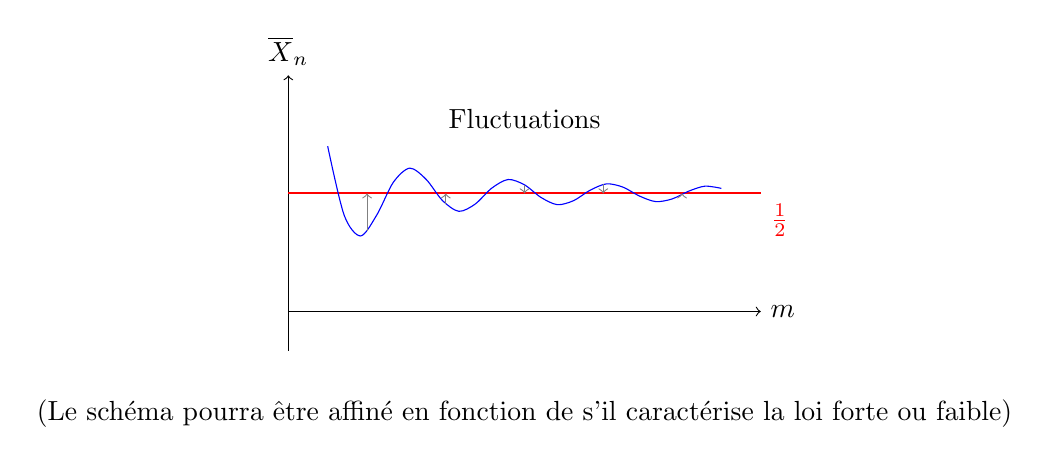
\begin{tikzpicture}
    % Axes
    \draw[->] (0,0) -- (6,0) node[right] {$m$}; % x-axis
    \draw[->] (0,-0.5) -- (0,3) node[above] {$\overline{X}_n$}; % y-axis
    
    % Horizontal line at 1/2
    \draw[thick, red] (0,1.5) -- (6,1.5) node[below right] {$\frac{1}{2}$};
    
    % Fluctuations curve
    \draw[domain=0.5:5.5, smooth, variable=\x, blue] plot ({\x}, {1.5 + 0.5*sin(5*\x r)/(\x)});
    \node[above] at (3, 2.2) {Fluctuations};
    
    % Arrows indicating stabilization
    \foreach \x in {1, 2, 3, 4, 5} {
        \draw[->, gray] (\x, {1.5 + 0.5*sin(5*\x r)/(\x)}) -- (\x, 1.5);
    }

    
    % Notes
    \node[below] at (3, -1)
    {(Le schéma pourra être affiné en fonction de s'il caractérise la loi forte ou faible)};
    
\end{tikzpicture}

\vspace{1cm}
Observons maintenant les fluctuations et la manière dont cela converge à travers le théorème central limite :

\section*{\underline{Théorème central limite}}


Le théorème central limite établit la convergence en loi de la somme d'une suite de variables aléatoires vers la loi normale.  

\vspace{0.3cm}
\noindent
Intuitivement, ce résultat affirme qu'une somme de variables aléatoires indépendantes et identiquement distribuées tend vers une variable aléatoire gaussienne.

\vspace{0.3cm}
\noindent
Ce théorème et ses généralisations offrent une explication de l'omniprésence de la loi normale dans la nature : de nombreux phénomènes sont dus à l'addition d'un grand nombre de petites perturbations aléatoires.

\vspace{0.3cm}
\noindent
Donnons d'abord une illustration avec le jeu de pile ou face, illustration ne nécessitant pas de connaissance particulière en statistique, mais uniquement en dénombrement. Il s'agit du même exemple que celui présent en introduction, seulement nous allons le ré-expliciter.

\vspace{0.3cm}
\noindent
Considérons le jeu de pile ou face et mettons des valeurs sur les faces de la pièce, par exemple 0 pour pile et 1 pour face ; on s'intéresse à la somme des tirages. La pièce est équilibrée, chaque face a une chance sur deux d'être tirée. Si l'on fait un seul tirage, alors le résultat peut être 0 ou 1, nous faisons la somme d'une seule valeur.



\section*{Résultat d'un tirage}

\begin{center}
\begin{tabular}{|c|c|c|}
\hline
Résultat tirage n° \( 1 \) & Somme \\ \hline
0 & 0 \\ \hline
1 & 1 \\ \hline
\end{tabular}
\end{center}

\textit{Nous avons donc ici 2 possibilités pour la valeur de la somme, qui apparaissent avec les fréquences suivantes :}

\begin{center}
\begin{tabular}{|c|c|c|}
\hline
Valeur de la somme & Nombre d'apparitions & Fréquence \\ \hline
0 & 1 & $\frac{1}{2} = 0,5$ \\ \hline
1 & 1 & $\frac{1}{2} = 0,5$ \\ \hline
\end{tabular}
\end{center}

\section*{Résultat de deux tirages}

\begin{center}
\begin{tabular}{|c|c|c|}
\hline
Résultat tirage n° \( 1 \) & Résultat tirage n° \( 2 \) & Somme \\ \hline
0 & 0 & 0 \\ \hline
0 & 1 & 1 \\ \hline
1 & 0 & 1 \\ \hline
1 & 1 & 2 \\ \hline
\end{tabular}

\vspace{0.3cm}

\begin{tabular}{|c|c|c|}
\hline
Valeur de la somme & Nombre d'apparitions & Fréquence \\ \hline
0 & 1 & $\frac{1}{4} = 0,25$ \\ \hline
1 & 2 & $\frac{2}{4} = 0,5$ \\ \hline
2 & 1 & $\frac{1}{4} = 0,25$ \\ \hline
\end{tabular}
\end{center}

\section*{Résultat de trois tirages}

\begin{center}
\begin{tabular}{|c|c|c|c|}
\hline
Résultat tirage n° \( 1 \) & Résultat tirage n° \( 2 \) & Résultat tirage n° \( 3 \) & Somme \\ \hline
0 & 0 & 0 & 0 \\ \hline
0 & 0 & 1 & 1 \\ \hline
0 & 1 & 0 & 1 \\ \hline
0 & 1 & 1 & 2 \\ \hline
1 & 0 & 0 & 1 \\ \hline
1 & 0 & 1 & 2 \\ \hline
1 & 1 & 0 & 2 \\ \hline
1 & 1 & 1 & 3 \\ \hline
\end{tabular}

\vspace{3 cm}


\begin{tabular}{|c|c|c|}
\hline
Valeur de la somme & Nombre d'apparitions & Fréquence \\ \hline
0 & 1 & $\frac{1}{8} = 0,125$ \\ \hline
1 & 3 & $\frac{3}{8} = 0,375$ \\ \hline
2 & 3 & $\frac{3}{8} = 0,375$ \\ \hline
3 & 1 & $\frac{1}{8} = 0,125$ \\ \hline
\end{tabular}
\end{center}

\vspace{1 cm}

\begin{figure}[H]
\centering
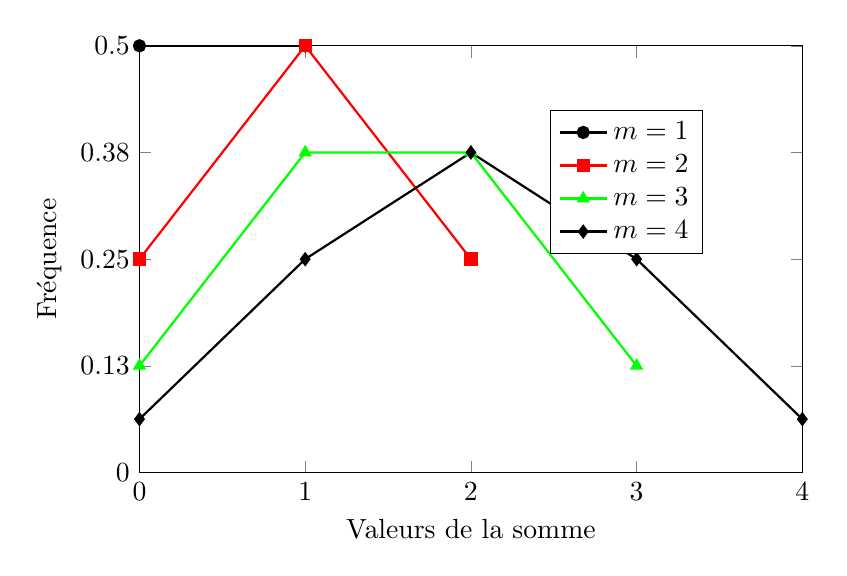
\begin{tikzpicture}
    \begin{axis}[
        width=10cm,
        height=7cm,
        xlabel={Valeurs de la somme},
        ylabel={Fréquence},
        ymin=0, ymax=0.5,
        xmin=0, xmax=4,
        xtick={0, 1, 2, 3, 4},
        ytick={0, 0.125, 0.25, 0.375, 0.5},
        legend style={at={(0.85,0.85)},anchor=north east},
        legend cell align={left}
    ]
    % Data for m=1
    \addplot[thick, mark=*] coordinates {
        (0, 0.5) (1, 0.5)
    };
    \addlegendentry{$m=1$}

    % Data for m=2
    \addplot[thick, mark=square*, color=red] coordinates {
        (0, 0.25) (1, 0.5) (2, 0.25)
    };
    \addlegendentry{$m=2$}

    % Data for m=3
    \addplot[thick, mark=triangle*, color=green] coordinates {
        (0, 0.125) (1, 0.375) (2, 0.375) (3, 0.125)
    };
    \addlegendentry{$m=3$}

    % Data for m=4
    \addplot[thick, mark=diamond*, color=black] coordinates {
        (0, 0.0625) (1, 0.25) (2, 0.375) (3, 0.25) (4, 0.0625)
    };
    \addlegendentry{$m=4$}
    \end{axis}
\end{tikzpicture}
\caption{Fréquence d'apparition d'une valeur pour la somme de tirages à pile ou face ($1 \leq m \leq 4$).}
\end{figure}


\section*{\underline{Énoncé du Théorème central limite}}

Soit $(X_n)_{n \in \mathbb{N}^*}$ une suite de variables aléatoires réelles indépendantes de même loi, d'espérance commune finie $m$ et de variance commune finie et non nulle $\sigma^2$. Pour $m \in \mathbb{N}^*$, on note :

\[
\overline{X}_n = \frac{S_n}{n} = \frac{1}{n} \sum_{k=1}^{n} X_k = \frac{X_1 + \ldots + X_n}{n}
\]
\noindent
Alors,

\[
Z_n = \frac{\overline{X}_n - \mathbb{E}(\overline{X}_n)}{\sqrt{\text{Var}(\overline{X}_n)}} = \frac{\overline{X}_n - m}{\sqrt{\sigma^2/n}} = \sqrt{n} \cdot \frac{\overline{X}_n - m}{\sigma} \xrightarrow[n \to \infty]{\mathcal{L}} \mathcal{N}(0,1).
\]

\noindent
En particulier, soit $F$ la fonction de répartition de la loi normale $\mathcal{N}(0,1)$, on a, pour tous réels $a, b$ avec $a < b$ :

\[
\mathbb{P}\left(a < Z_n < b\right) \xrightarrow[m \to \infty]{} \int_a^b \frac{1}{\sqrt{2\pi}} e^{-t^2/2} \, dt = F(b) - F(a).
\]

\noindent
Pour montrer la convergence en loi des variables aléatoires, on peut aussi montrer que les fonctions caractéristiques convergent simplement vers la fonction caractéristique de la gaussienne $\mathcal{N}(0,1)$.

\vspace{1cm}
\noindent
\textbf{Démonstration :}

\vspace{0.3cm}
\noindent

Soit $t \in \mathbb{R}$, alors :

\[
\varphi_{Z_n}(t) = \mathbb{E} \left( e^{it Z_n} \right) = \mathbb{E} \left( e^{it \left( \frac{\overline{X}_n - m}{\sqrt{\sigma^2 / n}} \right)} \right) = \mathbb{E} \left( e^{it \left( \sum_{k=1}^{n} \frac{X_k - m}{\sqrt{n \sigma^2}} \right)} \right)
\]

En notant $Y_k = \frac{X_k - m}{\sigma}$ pour tout $k = 1, \ldots, n$, on a  donc :

\[
\varphi_{Z_n}(t) = \mathbb{E} \left( e^{\frac{it}{\sqrt{n}} \sum_{k=1}^{n} Y_k} \right) = \mathbb{E} \left( \prod_{k=1}^{n} e^{\frac{it}{\sqrt{n}} Y_k} \right).
\]

Comme $Y_1, \ldots, Y_m$ sont des variables aléatoires indépendantes et de même loi, on a :

\[
\varphi_{Z_n}(t) = \prod_{k=1}^{n} \mathbb{E} \left( e^{\frac{it}{\sqrt{n}} Y_i} \right) = \left( \mathbb{E} \left( e^{\frac{it}{\sqrt{n}} Y_1} \right) \right)^n = \left( \varphi_{Y_1} \left( \frac{t}{\sqrt{n}} \right) \right)^n.
\]

\noindent
On peut alors faire un développement de Taylor-Young à l'ordre 2 pour $\varphi_{Y_1}$. En effet, $Y_1$ est de carré intégrable, et donc sa fonction caractéristique est deux fois dérivable en 0. On a :

\[
\varphi_{Y_1}'(0) = \mathbb{E}(Y_1) = 0 \quad \text{et} \quad \varphi_{Y_1}''(0) = -\mathbb{E}(Y_1^2) = -1.
\]

On a donc le développement limité suivant en 0 :

\[
\varphi_{Y_1}(u) = 1 - \frac{u^2}{2} + o(u^2) \quad \text{quand } u \to 0.
\]

En remplaçant $u$ par $\frac{t}{\sqrt{n}}$, on obtient pour tout réel $t$ :

\[
\varphi_{Y_1}\left(\frac{t}{\sqrt{n}}\right) = \varphi_{Y_1}(0) + \frac{t}{\sqrt{n}} \varphi_{Y_1}'(0) + \frac{t^2}{2n} \varphi_{Y_1}''(0) + o\left(\frac{1}{n}\right) \quad \text{quand } n \to \infty,
\]

ce qui donne :

\[
\varphi_{Y_1}\left(\frac{t}{\sqrt{n}}\right) = 1 + \frac{t}{\sqrt{n}} \cdot 0 - \frac{t^2}{2n} + o\left(\frac{1}{n}\right) = 1 - \frac{t^2}{2n} + o\left(\frac{1}{n}\right).
\]

En injectant cela dans l'égalité obtenue précédemment, on obtient :

\[
\varphi_{Z_n}(t) = \left( 1 - \frac{t^2}{2n} + o\left(\frac{1}{n}\right) \right)^n \quad \text{quand } n \to \infty.
\]

\noindent
À ce stade, on peut conclure en faisant tendre $n \to \infty$ si la quantité entre les parenthèses tend à valeurs réelles. Mathématiquement, les fonctions caractéristiques sont à priori à valeurs complexes (comme le cache astucieusement le $o\left(\frac{1}{n}\right)$), et il convient donc d'y réfléchir quelque peu.

\vspace{0.3cm}
\noindent
En fait, on a besoin de ce lemme:

\vspace{0.3cm}
\noindent
\textbf{Lemme :}

\vspace{0.3cm}
\noindent
Soit $(z_n)_{n \in \mathbb{N}^*}$ une suite à valeurs complexes. Si $\lim_{n \to \infty} z_n = z$, alors
\[
\left( 1 + \frac{z_n}{n} \right)^n \xrightarrow[n \to \infty]{} e^{z}.
\]
$t \rightarrow e^{-t^2/2}$ étant la fonction caractéristique de $\mathcal{N}(0,1)$, on a donc la convergence en loi de $(z_n)_{n \in \mathbb{N}^*}$ vers $\mathcal{N}(0,1)$.


\section*{\underline{Conclusion}}

En résumé, les théorèmes limites en probabilité occupent une place centrale en théorie de la probabilité et permettent de comprendre le comportement asymptotique de phénomènes totalement aléatoires. Ces outils servent ainsi de bases aux statistiques afin notamment d'effectuer des inférences fiables à partir d'échantillons observés, de quantifier l'incertitude, d'analyser la convergence des séquences aléatoires ou encore d'évaluer la probabilité d'événements rares ou fréquents.

\vspace{0.3cm}
\noindent
Omniprésents dans notre société, le rôle des théorèmes limites est crucial. Il va donc sans dire que la manière dont nous avons traité le sujet, n'est qu'une approche, une découverte des théorèmes limites, et qu'il existe encore bien d'autres raffinements, d'autres manières de s'en servir, ainsi que de les appréhender.

\bigskip
\bigskip 
\begin{flushright}
\textbf{BENSALAH Lockman}\\
\textbf{ISSAD Nassim}
\end{flushright}



\end{document}